\documentclass{article}

\usepackage[spanish]{babel}
\usepackage{wrapfig}
\usepackage{amsmath}
\usepackage{graphicx}
\usepackage[colorlinks=true, allcolors=blue]{hyperref}

\begin{document}
\begin{titlepage}
        \begin{figure}
            \vspace{-8 em}
            \hspace{-10 em}
            
\includegraphics[width=5cm]{ipn} \hfill 
\includegraphics[width=4cm]{escom}
            \hspace{-8 em}
        \end{figure}
        \begin{center}
            {\large Instituto Politécnico Nacional \par}
            {\Large Escuela Superior de Cómputo \par}
            \vspace{3cm}
            {\scshape\Huge Práctica 6: \\Programación Dinámica\\ \bfseries  \par}
            \vspace{3cm}
            {\itshape\Large Análisis de algoritmos \par}
            {\itshape\Large 3CV12 \par}
            \vfill
            {\Large Reyes Rodríguez Enrique Abdiel \par}
            {\Large Chávez Hernández Juan Diego \par}
            \vfill
            {\ \textit{abykings1@gmail.com} \par}
            {\ \textit{jdiegohdez0233@gmail.com} \par}
            \vfill
            {\Large Diciembre 2021\par}
        \end{center}
    \end{titlepage}
\newpage

    \textbf{Resumen: }
    En el siguiente trabajo se presenta el análisis a priori a un problema cuya solución implementada es dada con ayuda de la programación dinámica. \\
     
    \textbf{Palabras clave: } Algoritmo, complejidad, programación dinámica, LCS.
\section{Introducción}
    El siguiente trabajo presenta un problema cuya solución esta dada por el algoritmo LCS (Longest Common Subsequence) Cadena subsecuente más larga. Cuya solución se puede implementar con programación dinámica. Este también tiene una estructura óptima, es decir que el problema puede ser dividido en subproblemas más pequeños y simples, el cual puede ser dividido en subproblemas más simples. También tiene subproblemas que se traslapan: las soluciones de los subproblemas de nivel mayor utilizan soluciones de subproblemas menores. Los problemas con estas dos propiedades pueden ser resueltos por una técnica de programación llamada programación dinámica, en la que las soluciones de los subproblemas se almacenan en lugar de ser calculadas una y otra vez. Para ello, se necesita la técnica de memoización en la que se tabulan las soluciones de los subproblemas más pequeños para que esas soluciones se puedan utilizar para resolver el nivel más alto. \\
    Uno de los usos más comunes está en comparar archivos. El principio viene de la matriz que usamos en el algoritmo, ya que corresponde exactamente a las partes que van cambiando en las cadenas a comparar, corresponde a las partes que existen en la cadena uno y la cadena dos. \\
    La implementación de una solución recursiva sería ineficiente, ya que hay muchas llamadas repetidas. Esto provoca que las llamadas que tenemos, creen otras, dándonos un crecimiento exponencial. Por eso es que los resultados que vamos analizando, los vamos almacenando.\\ Se podria dividir el problema en 2. La parte donde se halla la LCS, que nos da como resultado una matriz con el mapa a seguir para hallar las ocurrencias y la parte donde se interpreta ese mapa.\\
    Como objetivo de la práctica está el mostrar el análisis de la complejidad temporal de un algoritmo que usa programación dinámica.\cite{1}
\section{Conceptos básicos}
    \textbf{Subsecuencia}\\
    Una subsecuencia es una subsecuencia que se deriva de otra, siendo que se pueden eliminar elementos, pero nunca cambiando su orden.\cite{2}\\
    \textbf{LCS}\\
    Se refiere a la subcadena con mayor número de elementos, respetando el orden.\cite{2}\\
    \textbf{Programación dinámica}\\
    Es un paradigma, en el cual su objetivo es el reducir el tiempo de ejecución, mediante los subproblemas superpuestos y subestructuras óptimas, apoyándose de la memoización para estos fines.\cite{3}\\
    \textbf{Memoizacion}\\
    La memoización es una técnica que se emplea en la programación dinámica. Se trata de una técnica de optimización que acelera el tiempo en que se ejecuta una solución, ahorrando cálculos, sirviendo esta como una memoria que almacena los datos que serán ocupados en un futuro.\cite{3}\\
   
 
    \textbf{Pseudocódigo implementado para el problema}
        \begin{verbatim}
            function lcs(x[] y[])
                m = x.length
                n = y.length
                l[m+1][n+1]
                for i=0, i<=m, i++
                    for j=0, j<=m, j++
                        if (i==0 || j==0) l[i][j]=0;
                        if (x[i-1] == y[j-1])
                            l[i][j] = l[i-1][j-1] +1
                        else
                            l[i][j] = max(l[i-1][j],l[i][j-1])
                return l
            
            function diff(x[], y[],i,j)
                l = lcs(x,y,i,j)
                while(i != 0 && j != 0)
                    if(i == 0)
                        additions+=y[j-1]         
                        j-=1;
                    if(j==0){
                        removals+=y[i-1]
                        i-=1
                    if(x[i-1] == y[j-1])
                        unchanged+=x[i-1]
                        i-=1
                        j-=1
                    if(l[i-1][j]<= l[i][j-1])
                        additions+=x[j-1]
                        j-=1
                    else
                        removals+=x[i-1]
                        i-=1
                    
            
        \end{verbatim}
        \newpage
\section{Experimentación y resultados}
    \subsection{Comparación de archivos}
    En este caso, solo se muestra la ejecición del programa.
    \begin{figure}[h!]
        \centering
        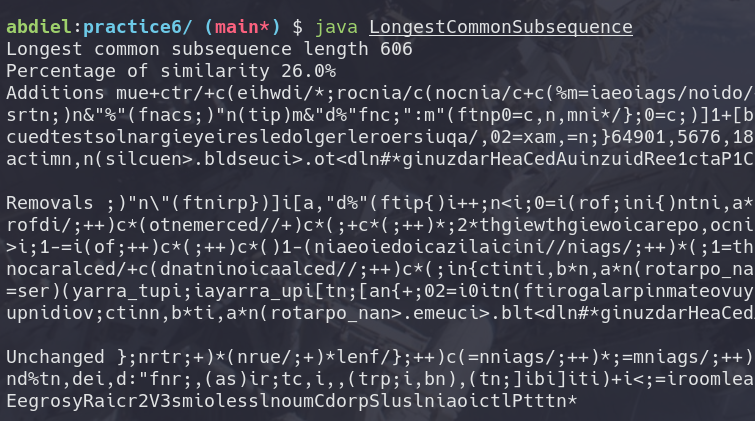
\includegraphics[width=1\textwidth]{p6_console_out.png}
        \caption{Esta es la compilacion y ejecucion de codigo en consola, donde se ven los caracteres que se añadieron, quitaron, o que no cambiaron. Asi mismo el porcentaje de similitud entre archivos}
        \label{fig:my_label}
    \end{figure}
    
\newpage
\section{Conclusiones}
    \begin{wrapfigure}{l}{0in}
        \centering
        
\includegraphics[scale=0.2]{abdiel.png}
    \end{wrapfigure}
    Enrique Abdiel Reyes Rodríguez:\\
    Con este paradigma me di cuenta de lo útil que es para dar soluciones eficaces , que no se compara a las soluciones que nos daría un  algoritmo voraz. Lo más complicado es trabajar con las matrices, ya que un error en un índice, puede ser un poco difícil de encontrar.
    Creo que el algoritmo provisto es una buena opción a elegir, y es una solución muy competente frente a otras.\\
    
    \begin{wrapfigure}{r}{0in}
        \centering
        
\includegraphics[scale=0.2]{diego.jpg}
    \end{wrapfigure}
    Juan Diego Chávez Hernández:\\
    A mi parecer, el desarrollo más complejo fue la forma de implementar la programación dinamica, ya que no estamos acostumbrados a los ejercicios con matrices.  Cabe mencionar que solo se realiza el analisis a priori y se comprueba que su orden es lineal, pero en terminos de las entradas que se le den. Pienso que seria interesante encontrar una solución más óptima, pero no logramos encontrar alguna.\\
    \newpage
    \newpage
\section{Anexo}
    \subsection{Análisis a priori del algoritmo utilizado }
    Tenemos 2 funciones encargadas de la comparación. Una es lcs, que nos crea una matriz donde están asignadas las comparaciones. Y diff, que trata las subcadenas que fueron cambiando. \\
    Analizando la primer funcion, vemos que hay 2 ciclos que se comportan de forma lineal. Estos pueden ir cambiando en función a sus límites, que son, m y n respectivamente. Las instrucciones que están dentro y fuera de los for son de orden constante y no alteran de forma alguna el comportamiento del algoritmo, por lo cual se tiene que \\
    $T(n) \in O(m*n)$\\
    Para la segunda función tenemos un ciclo while cual funciona como 2 ciclos for en simultaneo. Las instrucciones dentro y fuera de este ciclo son de orden constante y no alteran de forma alguna el comportamiento del algoritmo, por lo cual se tiene que\\
    $T(n) \in O(m + n)$\\
     \textbf{Pseudocódigo implementado para el problema}
        \begin{verbatim}
    function lcs(x[] y[])
        m = x.length --O(1)
        n = y.length --O(1)
        l[m+1][n+1] --O(1)
        for i=0, i<=m, i++ --O(m)
            for j=0, j<=m, j++ --O(n)
                if (i==0 || j==0) l[i][j]=0;--O(1)
                if (x[i-1] == y[j-1])       --O(1)
                    l[i][j] = l[i-1][j-1] +1--O(1)
                else
                    l[i][j] = max(l[i-1][j],l[i][j-1])--O(1)
        return l
    
    function diff(x[], y[],i,j)
        l = lcs(x,y,i,j)--O(1)
        while(i != 0 && j != 0)--O(m) y O(n) ---O(m + n)
            if(i == 0)
                additions+=y[j-1]--O(1)         
                j-=1;--O(1)
            if(j==0){
                removals+=y[i-1]--O(1)
                i-=1--O(1)
            if(x[i-1] == y[j-1])
                unchanged+=x[i-1]--O(1)
                i-=1--O(1)
                j-=1--O(1)
            if(l[i-1][j]<= l[i][j-1])--O(1)
                additions+=x[j-1]--O(1)
                j-=1--O(1)
            else
                removals+=x[i-1]--O(1)
                i-=1--O(1)
            
            
        \end{verbatim}
    
    \begin{figure}[h!]
        \centering
        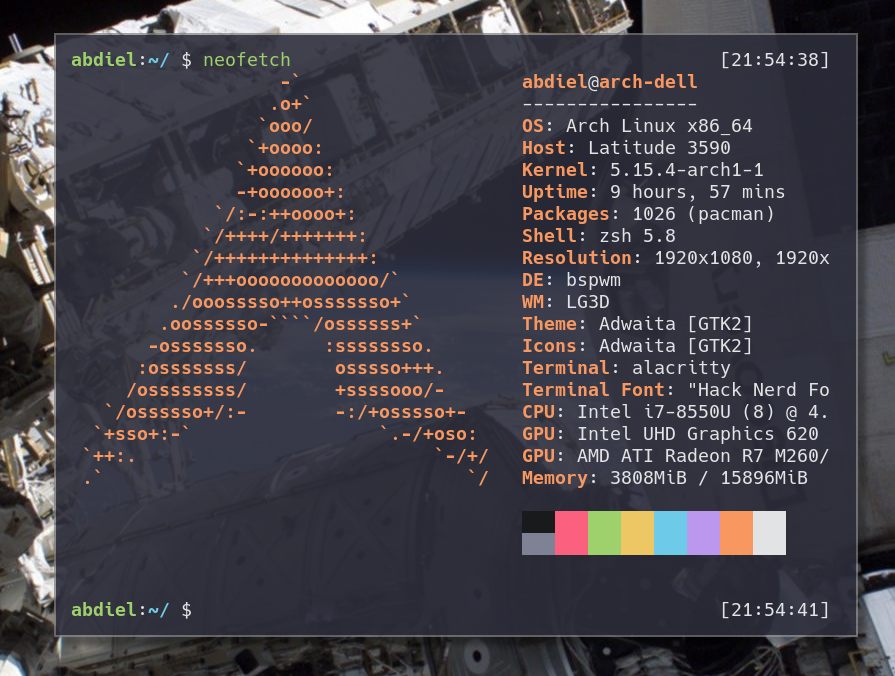
\includegraphics[width=0.9\textwidth]{specs.png}
        \caption{Estas son las especificaciones de la máquina en donde se ejecutó}
        \label{fig:my_label}
    \end{figure}
\newpage    
        
\begin{thebibliography}{}
    
        \bibitem{1}Cormen, T. H., Leiserson, C. E., Rivest, R. L., & Stein, C. (2009). Introduction to algorithms. MIT press.
        \bibitem{2}An Approach for Improving Complexity of Longest Common Subsequence Problems using Queue and Divide-and-Conquer Method. (2019, 1 mayo). IEEE Conference Publication | IEEE Xplore. Recuperado 3 de diciembre de 2021, de https://ieeexplore.ieee.org/document/8934638
        \bibitem{3}Bellman, R. (1966). Dynamic programming. Science, 153(3731), 34-37.

    \end{thebibliography}

\end{document}